\begin{question}
  \hspace*{\fill} [Note Maximale: 6]\par
  \noindent Soit $f(x)=p(x-q)(x-r)$.\par
  \medskip
  \begin{center} % or flushleft or flushright
    \noindent Une partie de la représentation graphique de $f$.\par
    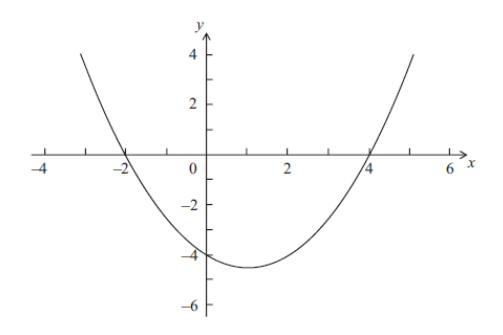
\includegraphics[scale=0.5]{figure_x10}\par
    \noindent La représentation graphique passe par les points $(-2; 0)$, $(0; -4)$ et $(4 ; 0)$\par
  \end{center} % or flushleft or flushright

  \begin{enumerate}[label=(\alph*)]
    \item Donnez la valeur de $q$ et de $r$.\hspace*{\fill} [2]
    \item Donnez l'équation de l'axe de symétrie.\hspace*{\fill} [1]
    \item Trouvez la valeur de $p$.\hspace*{\fill} [3]
  \end{enumerate}
\end{question}
